\chapter{Star Contraction}
\label{ch:graphcon::star}

\begin{preamble}
This chapter covers star partition and star contraction, an
efficient and parallel 
%
\href{def:graphcon::intro::graphcon::technique}{graph-contraction technique}
%
for general graphs. 
\end{preamble}

\section{Star Partition}
\label{sec:graphcon::star::partition}


In an 
%
\href{sec:graphcon::edge::partition}{edge partition},
%
if an edge incident on a vertex~$v$ is selected
as a block, then none of the other edges incident on $v$ can be their
own block.
%
This limits the effectiveness of the edge partition technique, because
it is unable to contract graphs with high-degree vertices
significantly.
%
In this section, we describe an alternative technique, star partition, that does not have this limitation.

\begin{flex}
\begin{definition}[Star Partition]
\label{def::graphcon::star-partition}
A~\defn{star partition} of a graph $G$ is a partition of $G$ where each block
is vertex-induced subgraph with respect to a 
%
\href{def:graphcon::edge::analysis::star::star-graph}{star graph}.
\end{definition}

\begin{example}
\label{ex:graphcon::star::partition::1}
Consider star graph with center $v$ and eight satellites.
  \begin{center}
  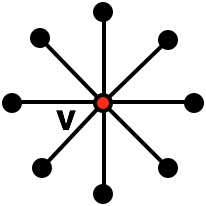
\includegraphics[width=1.5in]{./graph-contraction/media-star/star-graph1.jpg}
  \end{center}

\begin{itemize}
\item A partition consisting of the whole graph is a star partition, where 
the only block is the graph itself, induced by the star graph.

\item A partition where each block is an isolated vertex is a star
  partition, because each block is a vertex-induced subgraph of a
  single vertex, which is a star.
\end{itemize}

\end{example}


\begin{example}
\label{ex:graphcon::star::partition::2}


Consider the graph shown below on the left.
%
To partition this graph, we first find two disjoint stars, which are
highlighted.
%
Each star induces a block consisting of its vertices and the
corresponding edges of the graph.
%
These two blocks form a star partition the graph.
%
%% TODO: Comment this out in favor of the important block below.
Note that in a star partition, a block might not be a star.
\begin{center}
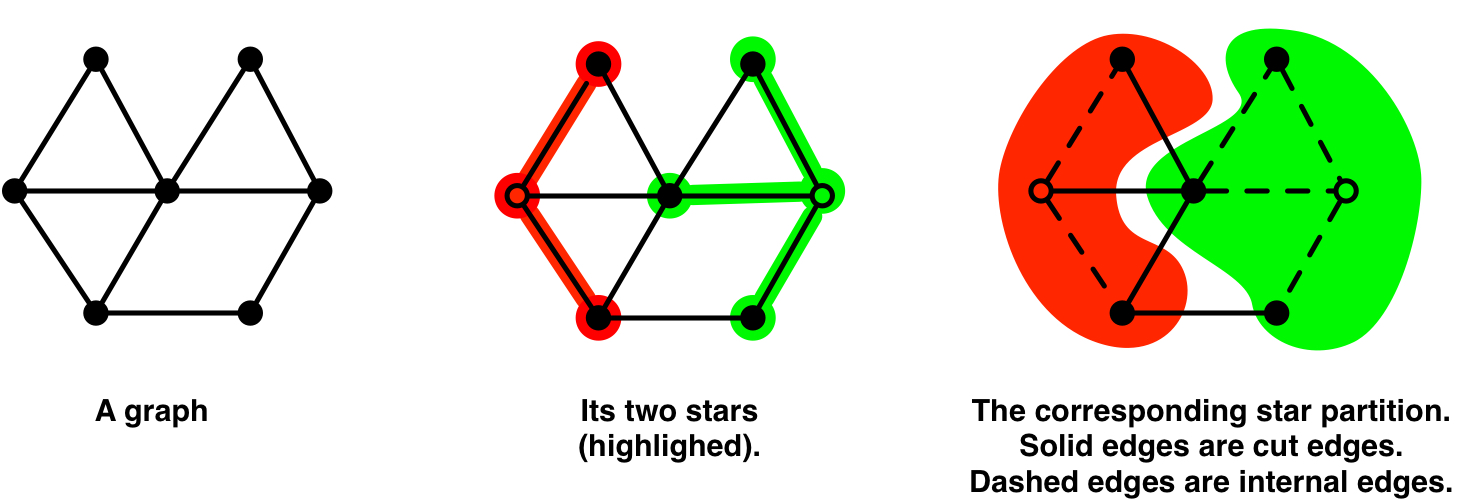
\includegraphics[width=0.9\textwidth]{./graph-contraction/media-star/star-decomposition-1.jpg}
\end{center}
\end{example}
\end{flex}

%% \begin{important}
%% In a star partition, a partition might not be a star.
%% \end{important}
%% \begin{teachask}
%% How can we star-partition a graph? 
%% \end{teachask} 

\begin{gram}[Constructing a Star Partition (Sequential)]
\label{graphcon::star::partition::seq}

We can construct a star partition sequentially by iteratively adding
stars until the vertices are exhausted as follows.

\begin{itemize}

\item Select an arbitrary vertex $v$ from the graph and make $v$ the
  center of a star.

\item Attach as satellites all the neighbors of $v$ in the graph.

\item Remove $v$ and its satellites from the graph.

\end{itemize}
%
\end{gram}

\begin{flex}
\begin{gram}[Computing a Star Partition (Parallel)]
\label{graphcon::star::partition::par}

We can construct a star partition in parallel by making local
independent decisions for each vertex, and using randomization to
break symmetry.
%
One approach proceeds as follows. 
%
\begin{itemize}
\item Flip a coin for each vertex.

\item If a vertex flips heads, then it becomes the center of a star. 
\item If a vertex flips tails, then there are two cases.
\begin{itemize}
\item The vertex has a neighbor that flips heads and the vertex selects the neighbor (breaking ties arbitrarily).  In this case, the vertex becomes a satellite.

\item The vertex doesn't have a neighbor that flips heads and it becomes a center. 
\end{itemize}
\end{itemize}

Note that if a vertex doesn't have a neighbor (it is ``isolated''), then it will always become a center. 
\end{gram}

\begin{definition}[Isolated Vertices]
\label{graphcon::star::partition::random::isolated}
We say that a vertex is \defn{isolated} in a graph if it doesn't have a neighbor.
\end{definition}

\begin{note}
The \href{graphcon::star::partition::par}{parallel approach}
%
to star partition is not optimal, because it might not always create
the smallest number of stars.
%
This is acceptable for us, because we only need to reduce the size of
the graph by some constant factor.
\end{note}

\begin{example}[Randomized Star Partition]
\label{ex:graphcon::star::partition::random}

The example below illustrates how we may partition a graph using the parallel star partition algorithm described above.
%
Vertices $\vname{a}$ and $\vname{b}$, which flip heads, become
centers. Vertices $\vname{c}$ and $\vname{e}$, which flipped tails,
attempt to become satellites by finding a center among their
neighbors, breaking ties arbitrarily.
%
If a vertex does not have a neighbor that is a center (flipped heads),
then it becomes a singleton star (e.g., vertex $d$).
%

The resulting star partition has three stars: the star with center $\vname{a}$ (with no
satellites), the star with center $\vname{b}$ (with two satellites),
and the singleton star $\vname{d}$.
%
The star partition thus yields three blocks, which are defined by the
subgraphs induced by each star.

\begin{center}
  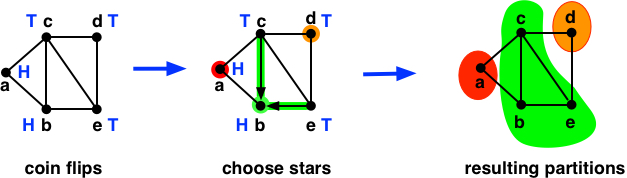
\includegraphics[width=6in]{./graph-contraction/media-star/star-find0.jpg}
\end{center}

\end{example}
\end{flex}


\begin{flex}
%require an undirected graph $G=(V,E)$ and round number $i$
%return $V'$ = remaining vertices after contraction,
%          $P$ = mapping from $V$ to $V'$
\begin{algorithm}[Parallel Star Partition]
\label{alg:graphcon::star-partition}

To specify the star-partition algorithm, we need
a source of randomness.
%
We assume that each vertex is given a (potentially infinite) sequence
of random and independent coin flips. The $i^{th}$ element of the
sequence can be accessed via the function
\[
\cheads~(v,i) : V \times \mathbb{Z} \to \mathbb{B}, 
\]
which returns $\cd{true}$ if the $i^{th}$ flip on vertex $v$ is heads
and false otherwise. 

The function $\cdvar{starPartition}$, whose pseudo-code is given
below, takes as argument a graph and a round number, and returns a
graph partition specified by a set of centers and a partition map from
all vertices to centers.
%

The algorithm starts by flipping a coin for each vertex and selecting
the edges that point from tails to heads---this gives the set of edges
$\mathit{TH}$.
%
In this set of edges, there can be multiple edges from the same
non-center. Since we want to choose one center for each satellite, we
remove duplicates in Line \linegcstarmerge{}, by creating a set of
singleton tables and merging them, which selects one center per
satellite.
%
This completes the selection of satellites and their centers. 
%

Next, the algorithm determines the set of centers as all the
non-satellite vertices.
%
To complete the process, the algorithm maps each center to itself
(Line~\linegcstarself{}).
%
These operations effectively promote unmatched non-centers to centers,
forming singleton stars, and matches all centers with themselves.
%
Finally, the algorithm constructs the
%
\href{def:graphcon::intro::prelim::partition-map}{partition map} 
%
by uniting the mapping for the satellites and the centers.
%

\[
\begin{array}{ll}
1 & \cdvar{starPartition}~(G=(V,E),i) =
\\
2 & ~~~~\cd{let}
\\
3 & ~~~~~~~~\cd{(* Find the arcs from satellites to centers. *)}
\\
4 & ~~~~~~~~\mathit{TH} = \csetf{(u,v) \in E}{\neg \cheads(u,i) \land \cheads(v,i)} %@\label{line:flip}\vspace{.1in}@
\\
5 & ~~~~~~~~\cd{(* Partition map: satellites map to centers *)}
\\
6 & ~~~~~~~~P_s = \bigcup_{(u,v) \in \mathit{TH}} \cset{u \mapsto v}
% \label{line:starmerge}
\\
7 & ~~~~~~~~\cd{(* Centers are non-satellite vertices *)}
\\
8 & ~~~~~~~~V_c = V \setminus \cdvar{domain}(P_s)
\\
9 & ~~~~~~~~\cd{(* Map centers to themselves *)}
\\
10 & ~~~~~~~~~P_c = \cset{u \mapsto u : u \in V_c} % \label{line:self}
\\
11 & ~~~~\cd{in}
\\
12 & ~~~~~~~~(V_c, P_s \cup P_c)
\\
13 & ~~~~\cd{end}
\end{array}
\]


\end{algorithm}

\begin{note}
\label{graphcon::star::partition::implementing-heads}

Since most machines don't have true sources of randomness, in practice
the function $\cdvar{heads}$ is usually implemented with a
pseudorandom number generator or with a good hash function.

In the algorithm, Line~\linegcstarmerge{} creates a set of
singleton tables and merges them.
%
This can be implemented using sets and tables as follows.
%
\[
\begin{array}{ll}
  \cdvar{Set.reduce}
  & (\cdvar{Table.union}~(\cfn{(x,y)}{x}))
\\
& \emptyset
\\
& \cset{\cset{u \mapsto v} : (u,v) \in \mathit{TH}}
\end{array}
\]
Note that we supply to the $\cdvar{union}$ operation a function that selects the first of the two possibilities; this is an arbitrary choice and we could have favored the second.

\end{note}

\begin{example}
\label{ex:graphcon::star::partition::alg}

Consider the star partition illustrated below.
\begin{center}
  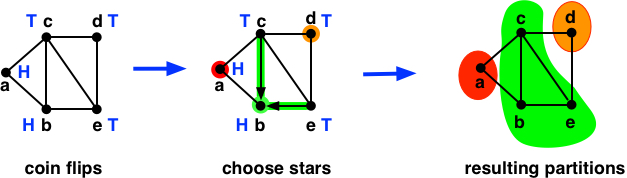
\includegraphics[width=6in]{./graph-contraction/media-star/star-find0.jpg}
\end{center}

The  star-partition algorithm proceeds on this example as follows.
%
First, it computes
%
\[
\mathit{TH} =
\cset{(\vname{c},\vname{a}),(\vname{c},\vname{b}),(\vname{e},\vname{b})},
\]
%
as the edges from satellites to centers.  
%
Now, it
converts each edge into a singleton table, and merges all the tables
into one
table, which is going to become a part of the partition map:
%
\[
P_s = \cset{\vname{c} \mapsto \vname{b},\vname{e} \mapsto \vname{b}}.
\]
%
Note that the edge $(\vname{c},\vname{a})$ has been removed since when
uniting the tables, we select only one element for each key in the
domain.  
%
Now for all remaining vertices
%
$V' = V \setminus \cdvar{domain}(P) = \cset{\vname{a},\vname{b},\vname{d}}$
we map them to themselves, giving:
%
\[
P_c = \cset{\vname{a} \mapsto \vname{a}, \vname{b} \mapsto \vname{b},
  \vname{d} \mapsto \vname{d}}.
\]
%
The vertices in $P'$ are the centers.
%
Finally we merge $P$ and $P'$ to obtain the partition map
%
\[
P_s \cup P_c = \cset{\vname{a} \mapsto \vname{a}, \vname{b} \mapsto \vname{b}, \vname{c} \mapsto \vname{b}, \vname{d} \mapsto
    \vname{d}, \vname{e} \mapsto \vname{b}}.
\]
\end{example}
\end{flex}


%% \begin{todo}
%% This theorem needs a proof.  What is the graph representation? 
%% It seems like it is an edge set representation.

%% The big union would require logn span do we need inject here?

%% \end{todo}

\begin{gram}[Implementation]
Suppose that we are given an enumerable graph with $n$ vertices and $m$ edges. 
%
We can represent the graph using 
%
\href{sec:graphs:graphs::edgesets}{an edge set representation}
%
and represent the sets with sequences.
%
This means that we have a sequence of vertices and a sequence of edges.
%

This representation enables a relatively clean implementation of the
%
\href{alg:graphcon::star-partition}{star-partition algorithm},
%
as shown by the pseudo-code below.
%
The implementation follows the pseudo-code for the algorithm but is able to compute the satellites and centers compactly by using a sequence $\cdvar{inject}$ operation.
%
The implementation first constructs a vertex sequence $V'$ where each vertex maps to itself.
%
It then constructs a sequence 
%
$\cdvar{TH}$ 
%
of ``updates'' from vertices that flip heads into tails,
%
and inject $\cdvar{TH}$ into the sequence of vertices $V'$.
%
The resulting sequence $P$ maps each vertex that flipped tails to  a center, if the vertex has a neighbor that flipped heads.
%
The sequence $P$ ensures that a vertex that has flipped heads  remains unaffected by the injection, e.g., if vertex $i$ has flipped heads, then 
%
$P[i] = i$.
%
We can thus compute set of centers by filtering over $P$ and use the sequence $P$ to represent the partition map for satellites and centers jointly.
\[
\begin{array}{l}
\cdvar{starPartition}~(G = (V, E), i) =
\\
~~~~\cd{let}
\\
~~~~~~~~~V' = \cseq{i : 0 \le i < |V|}
\\
~~~~~~~~~\cdvar{TH} = \cseq{ (u,v) \in E \sucht \neg \cheads~(u, i), \cheads~(v, i) }
\\
~~~~~~~~~P = \cdvar{Seq.inject}~V'~TH
\\
~~~~~~~~~V_C = \cdvar{Seq.filter}~(\cd{lambda}~i.~P[i] = i)~P
in (V_C, P) end
\end{array}
\]
\end{gram}

\subsection{Analysis of Star Partition}
\label{sec:graphcon::star::partition::analysis}


\begin{theorem}[Cost of Star Partition]
\label{thm:graphcon::star::partition::analysis}
Based on the array-based cost specification for sequences, the cost of $\cdvar{starPartition}$ is 
\[
O(n + m)
\]
work and 
\[
O(\lg n)
\]
span for a graph with $n$ vertices and $m$ edges.
\end{theorem}

\begin{exercise}
Prove the theorem.
\end{exercise}

\begin{teachask}
 In expectation, how big is $P$?  
\end{teachask}


\begin{gram}[Number of Satellites]
\label{graphcon::star::partition::analysis::nsat}

Let us also bound the number of satellites found by
$\cdvar{starPartition}.$
%
Note first that there is a one-to-one mapping between the satellites
and the set $P_s$ computed by  the algorithm.
%
%
The following lemma establishes that on a graph with
$\nn$~non-isolated vertices, the number of satellites is at least
$\nn/4$ in expectation.
%
As we will see this means that we can use star partition to perform
graph contraction with logarithmic span.
\end{gram}

\begin{flex}
\begin{lemma}[Number of Satelites]
\label{lem:graphcon::star::partition::analysis::satellites}
  For a graph $G$ with $\nn$ non-isolated vertices, the expected
  number of satellites in a call to $\cdvar{starPartition}~(G,i)$ with
  any~$i$ is at least $\nn/4$.
\end{lemma}

\begin{proof}
  For any vertex $v$, let $H_v$ be the event that a vertex $v$ comes
  up heads, $T_v$ that it comes up tails, and $R_v$ that $v \in
  \cdvar{domain}(P)$ (i.e, it is a satellite).
%
  Consider any non-isolated vertex $v \in V(G)$.  By definition, we
  know that a non-isolated vertex $v$ has at least one neighbor $u$.
  So, we know that $T_v \land H_u$ implies $R_v$, since if $v$ is a
  tail and $u$ is a head $v$ must either join $u$'s star or some other
  star.  Therefore, $\prob{R_v} \geq \prob{T_v} \prob{H_u} = 1/4$.  By
  the linearity of expectation,  the expected number of satellites is
  \begin{align*}
    \expct{\sum_{v: v \text{ non-isolated}} \onef{R_v}} & = \sum_{v: v
      \text{ non-isolated}} \expct{\onef{R_v}} 
\\[2mm]
  & \geq \nn/4.
  \end{align*}
  The final inequality follows because we have $\nn$ non-isolated
  vertices and because the expectation of an indicator random variable
  is equal to the probability that it takes the value $1$.
\end{proof}
\end{flex}

\begin{teachnote}
Consider the random variable that a vertex becomes a satellite.  This
happens if the vertex flips tails and it has a neighbor that flips
heads.  A non-isolated vertex has at least one neighbor, therefore
this probability is at least 1/4.  The bound follows.
\end{teachnote}


\section{Star Contraction}
\label{sec:graphcon::star::contract}

\begin{definition}[Star Contraction]
\label{def:graphcon::star-contraction}
\defn{Star contraction} is an instance of graph contraction that uses
star partitions to contract the graph.
\end{definition}

\begin{algorithm}[Star Contraction]
\label{alg:graphcon::star-contraction}

The pseudo-code below gives a higher-order
star-contraction algorithm.
%
The algorithm takes as arguments the graph $G$ and two functions:
\begin{itemize}
\item  $\cdvar{base}$ function specifies the computation in the base case, and

\item  $\cdvar{expand}$ function computes the result for the larger
graph from the quotient graph.

\end{itemize}


In the base case, the graph contains no edges and the function
$\cdvar{base}$ is called on vertex set.

In the recursive case, the graph is partitioned by a call to
%
\href{alg:graphcon::star-partition}{star partition} 
(Line~\linegcscpartition{}),
%
which  returns the set of (centers) super-vertices
$V'$ and $P$ the
%
\href{def:graphcon::intro::prelim::partition-map}{partition map}
%
mapping every $v \in V$ to a $v' \in V'$.
%
The set $V'$ defines the super-vertices of the quotient graph.
%
Line~\linegcscedges{} computes the edges of the quotient graph by
routing the end-points of each edge in $E$ to the corresponding
super-vertices in $V'$ as specified by partition-map $P$.
%
Note that the filter $\cget{P}{u} \neq \cget{P}{v}$.
removes self edges.
%
The algorithm then recurs on the quotient graph $(V', E')$.
%
The algorithm then computes the result for the whole graph by calling
the function $\cdvar{expand}$ on the result of the recursive call $R$.

%
%%%% Doesn't belong here.
%% In the base case, each connected component has been contracted down to
%% a singleton vertex, and thus the number of vertices in the contracted
%% graph is equal to the number of components in the input graph.


\[
\begin{array}{ll}
1 & \cdvar{starContract}~\cdvar{base}~\cdvar{expand}~(G = (V,E)) =
\\ 
2 & ~~~~\cd{if}~|E| = 0~\cd{then}
\\
3 & ~~~~~~~~\cdvar{base}~(V)
\\
4 & ~~~~\cd{else}
\\ 
5 & ~~~~~~~~\cd{let}
\\ 
6 & ~~~~~~~~~~~~(V',P) = \cdvar{starPartition}~(V,E)~ % @\label{line:graphcon::cc::partition}@
\\
7 & ~~~~~~~~~~~~E' = \csetf{(\cget{P}{u},\cget{P}{v}) : (u,v) \in  E}{\cget{P}{u} \neq \cget{P}{v}} 
% @\label{line:graphcon::cc::edges}@
\\
8 & ~~~~~~~~~~~~R = \cdvar{starContract}~\cdvar{base}~\cdvar{expand}~(V',E')
\\
9 & ~~~~~~~~\cd{in}
\\
10 & ~~~~~~~~~~~~\cdvar{expand}~(V, E, V', P, R)
\\
11 & ~~~~~~~~\cd{end}
\end{array}
\]

\end{algorithm}

\begin{teachnote}
TODO [this is somewhat resolved]
This analysis is rather imprecise, because we have not written the
pseudocode for graph contraction.  How do we re-route edges and such.
This should be done.
\end{teachnote}

\begin{flex}
\begin{theorem}[Work and Span of Star Contraction]
\label{thm:graphcon::star-contraction-cost}
  For a graph $G = (V,E)$, we can contract the graph into a number of
  isolated vertices in $O\left((|V| + |E|) \lg |V|\right)$ work and $O(\lg^2 |V|)$ span.
\end{theorem}

For the proof, we will consider work and span separately
%
and assume that
%
\begin{itemize}
   \item function $\cdvar{base}$ has constant span and linear work in the
     number of vertices passed as argument, and
\item function $\cdvar{expand}$ has linear work and logarithmic span in
  the number of vertices and edges at the corresponding step of the
  contraction.
  \end{itemize}

\begin{gram}[Span of Star Contraction]
\label{graphcon::star::contraction::cost::proof::span}
Let $\nn$ be the number of non-isolated vertices.
%
In star contraction, once a vertex becomes isolated, it remains
isolated until the final round, since contraction only removes edges.
%
Let $\nn'$ denote the number of non-isolated vertices after one round of star
contraction.
%
We can write the following recurrence for the span of star contraction.
%
\[
\begin{array}{lll}
S(\nn)  & = &
\left\{
\begin{array}{lll}
S(\nn') + O(\lg n) & \mbox{if} & \nn > 0
\\
1 & \mbox{otherwise.}
\end{array}
\right.
\end{array}
\]
%

Observe that $\nn' = \nn - X$, where $X$ is the number of satellites
(as defined earlier in the lemma about $\cdvar{starPartition}$), which are
removed at a step of contraction. Since $\expct{X} = \nn/4$,
$\expct{\nn'} = 3n/4$.
%
This is a familiar recurrence, which we know solves to $O(\lg^2
\nn)$, and thus $O(\lg^2 n)$, in expectation.
\end{gram}


\begin{gram}[Work of Star Contraction]
\label{graphcon::star::contraction::cost::proof::work}
For work, we would like to show that the overall work is linear,
because we might hope that the graph size is reduced by a constant
fraction on each round.
%
Unfortunately, this is not the case.  Although we have shown that star
contraction can remove a constant fraction of the non-isolated
vertices in one round, we have not bounded the number of edges
removed.
%

%% \begin{teachask}
%% How many edges can we remove? 
%% \end{teachask}
%
Because removing a satellite also removes the edge that attaches it to
its star's center, each round  removes at least as many edges as vertices.  
%
But this does not help us bound
the number of edges removed by a linear function of $m$, because there
can be as many an $n^2$ edges in the graph.
%
%% This is confusing.
% Thus, all we know is that there are at least $m-n$ edges after one
% round of contraction.

To bound the work, we will consider non-isolated and isolated vertices
separately.
%
Let $\nn'$  denote the  number of non-isolated vertices after one
round of star contraction.
%
For the non-isolated vertices, we have the following work recurrence:
\[
\begin{array}{lll}
W(\nn, m) 
\leq 
\left\{
\begin{array}{lll}
W(\nn', m) + O(\nn+m) & \mbox{if} & \nn > 1
\\
1 & \mbox{otherwise.}
\end{array}
\right.
\end{array}
\]
%
This recursion solves to
\[
\expct{W(\nn,m)} = O(\nn + m\lg \nn) = O(n + m \lg{n}).
\]

To bound the work on isolated vertices, we note that there at most $n$
of them at each round and thus, the additional work is $O(n \lg{n}).$

We thus conclude that the total work is
\[
O((n + m)\lg{n}).
\]
\end{gram}

\begin{note}
Consider as an example a star contraction where $n$ and $m$ have the
following values in each round.
\[
\begin{array}{lll}
\hline
 \mbox{round} & \mbox{vertices} & \mbox{edges}
\\
\hline
 1 & n & m 
\\
 2 & n/2 & m - n/2 
\\
 3 & n/4 & m - 3n/4 
\\
 4 & n/8 & m - 7n/8 
\\
\hline
 \end{array}
\]
It is clear that the number of edges does not drop below $m-n,$ so if
there are $m > 2n$ edges to start with, the overall work will be $O(m
\lg n)$.
%
\end{note}
%
\end{flex}

\begin{teachnote}
Note that if the graph is complete, we do actually reduce the number
of edges by a constant fraction be eliminating redundancy, because we
can only have so many edges in the quotient graph. This brings up an
interesting point about when this algorithm actually performs poorly.
It might be interesting to study some real world instance.
\end{teachnote}

\begin{teachnote}
Idea: Consider a contraction along with the randomness function.
Consider each round and the blocks contracted in that round.
Add just as many edges as possible (without leading to duplicates)
between those blocks.  Make sure that you don't generate duplicates
in following rounds.  Since each block is nested inside a
logarithmic number of other blocks.  It is possible to construct
such a graph that also has a large number of edges.
\end{teachnote}

